\begin{ExerciseList}
\section{Lab 1: Booting a PC}

\subsection{实验简介}

本实验被分为三个部分。第一个部分主要集中在熟悉x86汇编语言、QEMU模拟器以及PC的启动步骤。第二个部分通过实践来对系统内核的boot loader进一步了解。第三部分来深入研究JOS的系统内核。

\subsection{实验目的}

\begin{enumerate}
\item 熟悉(复习)x86汇编语言,为接下来的工作打好基础
\item 了解开发环境的使用方法,尤其是QEMU模拟器的使用
\item 对PC启动的过程有更清晰的了解
\item 了解堆栈,清楚函数调用时的栈帧结构
\end{enumerate}

\subsection{实验内容}

\subsubsection{准备}

装完QEMU模拟器之后,如果想做后续的实验,还需要下载JOS的残缺的源码(需要我们在后面填充内容)。

\shell{git clone https://pdos.csail.mit.edu/6.828/2017/jos.git lab}
\shell{cd lab}

进入lab目录之后,如图\ref{fig:lab1:jos},我们可以看到lab目录的大致结构。

\begin{figure}[H]
  \centering
  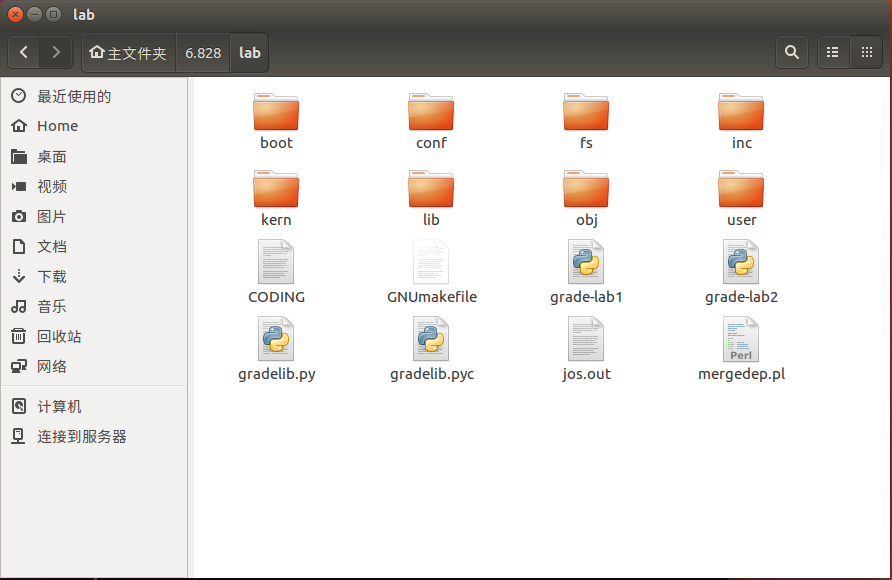
\includegraphics[width=6in]{figures/lab1/jos.png}
  \caption{lab目录的结构}\label{fig:lab1:jos}
\end{figure}

在lab目录下运行如下命令:

\shell{make qemu}

如图\ref{fig:lab1:make_qemu},就能用QEMU运行JOS。

\begin{figure}[H]
  \centering
  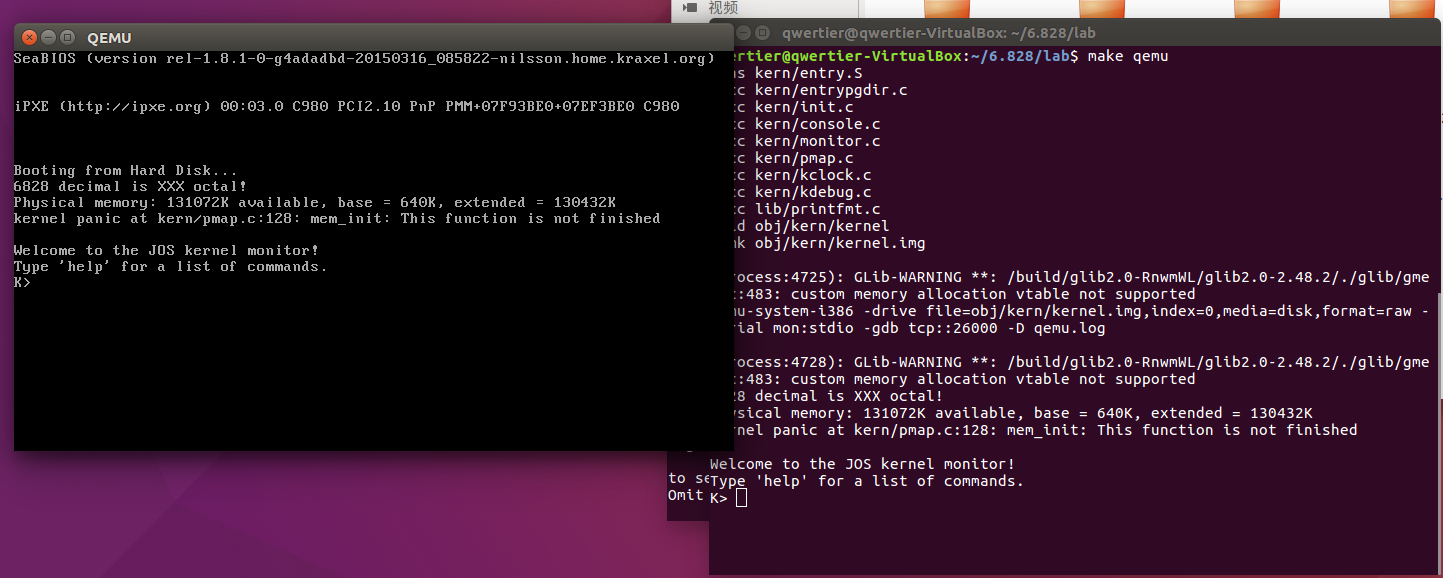
\includegraphics[width=6in]{figures/lab1/make_qemu.png}
  \caption{lab目录的结构}\label{fig:lab1:make_qemu}
\end{figure}

\subsubsection{第一部分:启动PC}

\Exercise{熟悉汇编语言}

汇编语言的英文资料可以在\url{https://pdos.csail.mit.edu/6.828/2017/reference.html}找到。

\Exercise{使用GDB的单步调试(si)语句追踪ROM BIOS,然后猜测它在做什么。}

在一个终端中输入 make qemu-gdb , 另一个终端输入 make gdb 。开始调试程序。

\shell{[f000:fff0] 0xffff0: ljmp \$0xf000,\$0xe05b}

是GDB反汇编出的第一条执行指令,这条指令表明了:IBM PC 执行的起始物理地址为 0x000ffff0,PC 的偏移方式为 CS = 0xf000,IP = 0xfff0。

\begin{figure}[H]
  \centering
  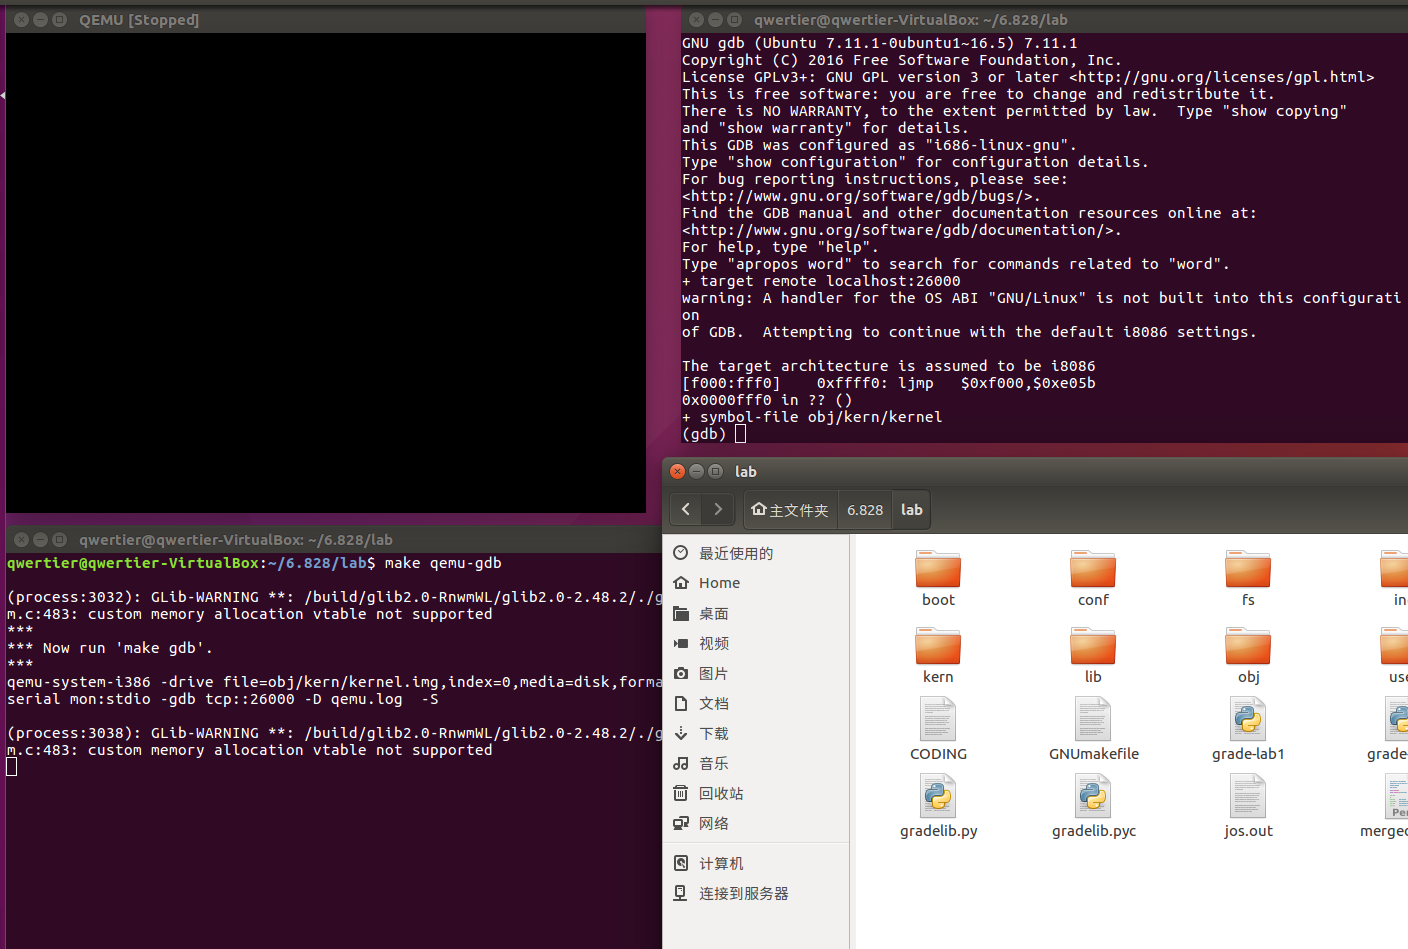
\includegraphics[width=6in]{figures/lab1/gdb.png}
  \caption{使用gdb调试第一条指令}\label{fig:lab1:gdb}
\end{figure}

第一条指令执行的是 jmp指令,跳转到段地址 CS = 0xf000,IP = 0xe05b。QEMU模拟了8088处理器的启动,当启动电源,BIOS最先控制机器,这时还没有其他程序执行,之后处理器进入实模式也就是设置 CS 为 0xf000,IP 为 0xfff0。在启动电源也就是实模式时,地址转译根据这个公式工作:物理地址 = 16 * 段地址 + 偏移量。所以 PC 中 CS 为 0xf000 IP 为 0xfff0 的物理地址为:

\begin{align}
   & 16 * 0xf000 + 0xfff0\\
   = & 0xf0000 + 0xfff0\\
   = & 0xffff0
\end{align}

0xffff0 在 BIOS (0x100000) 的结束地址之前。

当BIOS开始运行时,它会建立中断描述表\footnote{Interrupt Descriptor Table}然后初始化众多设备(例如显示器)。这就是当你从QEMU中看到''Starting SeaBIOS''的时候。

当所有的其他设备都初始化完成了,BIOS会继续找可以启动的设备(例如硬盘、CD-ROM)。最后它会找到可启动盘,接着BIOS从启动盘中读出boot loader然后转移控制权。

\subsubsection{第二部分:The Boot Loader}

\Exercise{在\url{https://pdos.csail.mit.edu/6.828/2017/labguide.html}熟悉一下 GDB 的指令。然后在0x7c00处设一个断点,执行到断点。进入boot/boot.S,参考源代码和反汇编代码 \emph{obj/boot/boot.asm}来跟踪。追踪到bootmain函数中,而且还要具体追踪到readsect()子函数里面。找出和readsect()c语言程序的每一条语句所对应的汇编指令,回到bootmain(),然后找出把内核文件从磁盘读取到内存的那个for循环所对应的汇编语句。找出当循环结束后会执行哪条语句,在那里设置断点,继续运行到断点,然后运行完所有的剩下的语句。}

\textbf{\$[0:7c2d] => 0x7c2d: ljmp \$0x8,\$0x7c32}这条指令之后,也就是 boot.S 中的\textbf{ ljmp \$PROT\_MODE\_CSEG, \$protcseg} ,地址符号就变成 0x7c32 了。

首先查看boot.S文件,在开头可以看到如下代码,cld 是串操作指令,用来操作方向标志位DF,使DF=0。

\begin{minted}{ASM}
start:
  .code16
  cli
  cld                         # String operations increment
\end{minted}

如以下代码,\textbf{inb \$0x64,\%al}把$0x64$端口(8042键盘控制器)的状态写入al中(inb代表IO端口读), 之后 \textbf{testb \$0x2,\%al}判断al的第二位是否为0,不为0就循环执行seta20.1。这里第二位代表输入缓冲区是否满了。接着$0xd1$放入$0x64$端口。最后将$0xdf$放入0x60端口,代表开启A20地址线了。

\begin{minted}{ASM}
  # Enable A20:
  #   For backwards compatibility with the earliest PCs, physical
  #   address line 20 is tied low, so that addresses higher than
  #   1MB wrap around to zero by default.  This code undoes this.
seta20.1:
  inb     $0x64,%al               # Wait for not busy
  testb   $0x2,%al
  jnz     seta20.1

  movb    $0xd1,%al               # 0xd1 -> port 0x64
  outb    %al,$0x64

seta20.2:
  inb     $0x64,%al               # Wait for not busy
  testb   $0x2,%al
  jnz     seta20.2

  movb    $0xdf,%al               # 0xdf -> port 0x60
  outb    %al,$0x60
\end{minted}

通过如下代码,开始调用\emph{bootmain}函数。

\begin{minted}{ASM}
  # Set up the stack pointer and call into C.
  movl    $start, %esp
  call bootmain
\end{minted}

如下代码所示,在bootmain函数中,调用readseg函数。该函数有三个参数,分别是物理地址、页大小和偏移量。

\begin{minted}{ASM}
  # read 1st page off disk
  readseg((uint32_t) ELFHDR, SECTSIZE*8, 0);
    push   $0x0
    push   $0x1000
    push   $0x10000
    call   7cdc <readseg>
\end{minted}

如下指令用于加载程序段。

\begin{minted}{ASM}
    mov    0x1001c,%eax
    movzwl 0x1002c,%esi
    lea    0x10000(%eax),%ebx
    shl    $0x5,%esi
    add    %ebx,%esi
\end{minted}

\Exercise{了解C语言中关于指针的知识(已经学过了)}

为了理解 boot/main.c, 需要了解ELF二进制文件。编译并链接比如JOS内核这样的C程序,编译器会将源文件(.c)转为包含汇编指令的目标文件(.o)。接着链接器把所有的目标文件组合成一个单独的二进制镜像(binary image),比如 obj/kern/kernel,这种文件就是ELF(是可执行可链接形式的缩写)。

当前只需要知道,可执行的ELF文件由带有加载信息的头,多个程序段表组成。每个程序段表是一个连续代码块或者数据,它们要被加载到内存具体地址中。boot loader 不修改源码和数据,直接加载到内存中并运行。

ELF开头是固定长度的 ELF头,之后是一个可变长度的程序头,它列出了需要加载的程序段。ELF头的定义在 inc/elf.h 中。主要学习以下3个程序段:

\begin{itemize}
\item .text: 程序执行指令
\item .rodata:只读数据,比如ASCII字符串
\item .data: 存放程序初始化的数据段,比如有初始值的全局变量。
\end{itemize}

使用以下命令可以查看\emph{obj/kern/kernel}文件的ELF头的相关信息,结果如图\ref{fig:lab1:kernel_elf}。

\shell{objdump -h obj/kern/kernel}

\begin{figure}[H]
  \centering
  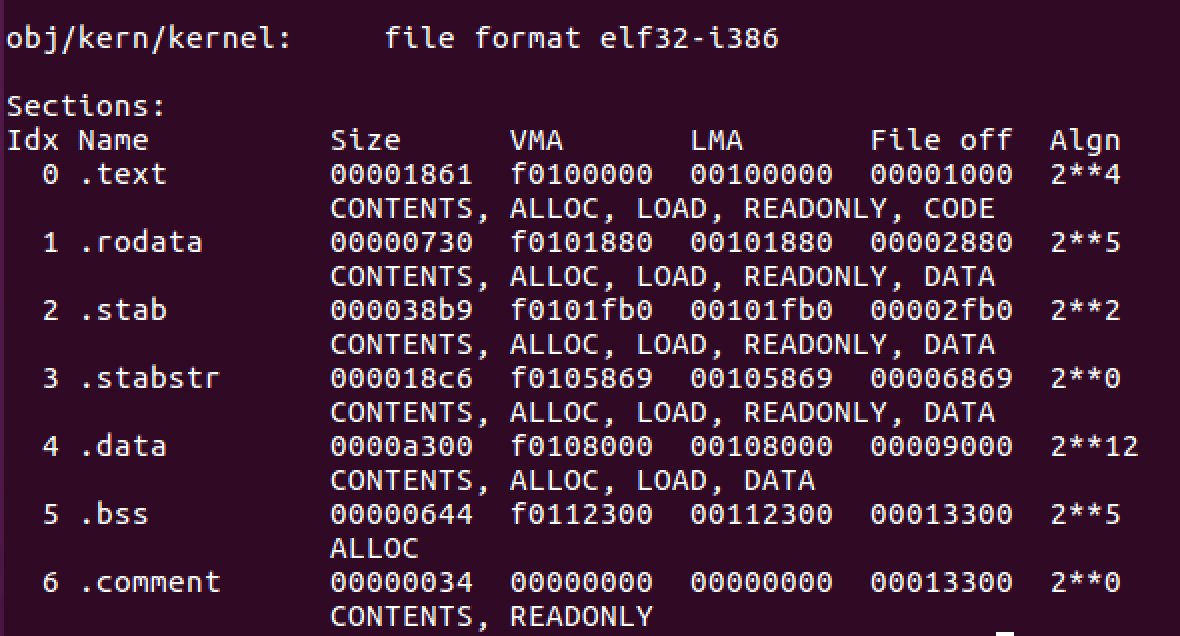
\includegraphics[width=6in]{figures/lab1/kernel_elf.png}
  \caption{\emph{obj/kern/kernel}文件的ELF头}\label{fig:lab1:kernel_elf}
\end{figure}

使用以下命令可以查看\emph{obj/boot/boot.out}文件的ELF头的相关信息,结果如图\ref{fig:lab1:boot_elf}所示。

\shell{objdump -h obj/boot/boot.out}

\begin{figure}[H]
  \centering
  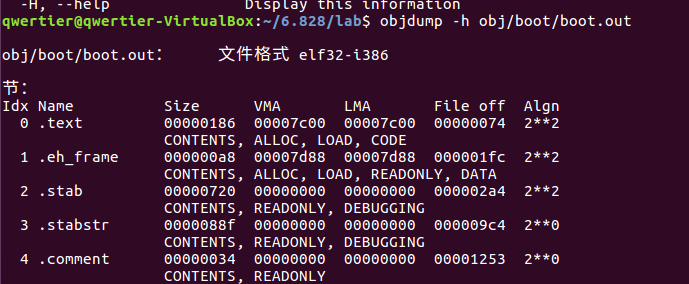
\includegraphics[width=6in]{figures/lab1/boot_elf.png}
  \caption{\emph{obj/boot/boot.out}文件的ELF头}\label{fig:lab1:boot_elf}
\end{figure}

\Exercise{修改\emph{boot/Makefrag},使得boot loader的加载地址出错,找到第一条出错的指令。\footnote{做完之后需要使用\textbf{make clean}命令之后再make。}}

查看\emph{boot/Makefrag}文件,文件内容如下所示。可以发现\textbf{-Ttext}后面的参数就是入口地址。如果把这个值修改为$0x8C00$,保存后回到lab1文件夹下进行make。

\begin{minted}{Makefile}
$(OBJDIR)/boot/boot: $(BOOT_OBJS)
    @echo + ld boot/boot
    $(V)$(LD) $(LDFLAGS) -N -e start -Ttext 0x7C00 -o $@.out $^
    $(V)$(OBJDUMP) -S $@.out >$@.asm
    $(V)$(OBJCOPY) -S -O binary -j .text $@.out $@
    $(V)perl boot/sign.pl $(OBJDIR)/boot/boot

\end{minted}

如下代码,查看\emph{obj/boot/boot.asm}会发现起始地址从原来的00007c00 变为 00008c00。虽然此时在0x7c00处打断点然后运行时正常的,但是继续si以后会在 \textbf{[0:7c2d] => 0x7c2d: ljmp \$0x8,\$0x8c32} 出循环,同时qemu端口出现了错误。因为不能ljmp到\$0x7c32而是调到了\$0x8c32,所以无法执行正确的指令。查看 boot.asm 可以知道上面这个指令是 \textbf{ljmp \$PROT\_MODE\_CSEG, \$protcseg},是为了进入32位模式的。

\begin{minted}{ASM}
.set CR0_PE_ON,      0x1         # protected mode enable flag

.globl start
start:
  .code16                     # Assemble for 16-bit mode
  cli                         # Disable interrupts
    8c00:    fa                       cli
  cld                         # String operations increment
    8c01:    fc                       cld
\end{minted}

\Exercise{使用GDB的\textbf{x}\footnote{参考\url{https://sourceware.org/gdb/current/onlinedocs/gdb/Memory.html}}命令可以可以查看内存信息。重启QEMU,当BIOS进入boot loader时检查0x00100000处的8个字节,然后在boot loader进入内核时再看一次。为什么两者有不同?在第二个端点处到底有什么?}

在0x7c00处设置断点,然后运行到断点处,使用 x/8x 0x100000 可以看到如图\ref{fig:lab1:gdb_x}

\begin{figure}[H]
  \centering
  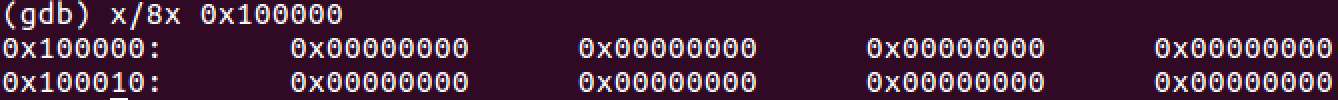
\includegraphics[width=6in]{figures/lab1/gdb_x.png}
  \caption{内存截图}\label{fig:lab1:gdb_x}
\end{figure}

根据之前的看到程序入口点是 0x10000c ,所以在 0x10000c 处打断点运行,如图\ref{fig:lab1:gdb_x2}同样可以看到

\begin{figure}[H]
  \centering
  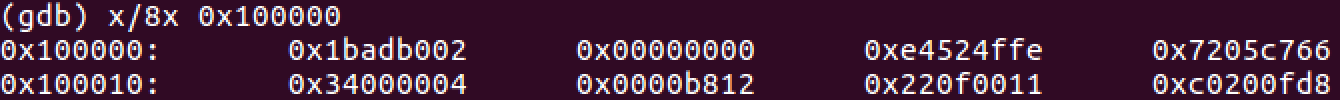
\includegraphics[width=6in]{figures/lab1/gdb_x2.png}
  \caption{内存截图}\label{fig:lab1:gdb_x2}
\end{figure}

$0x100000$处存放的其实就是程序指令段,也就是说 bootmain 函数会把内核的程序段送到内存$0x100000$处。



\subsubsection{第三部分:内核}

boot loader 的链接地址和加载地址是一样的,然而 kernel 的链接地址和加载地址有些差异。查看 kern/kernel.ld 可以发现内核地址在 0xF0100000。

操作系统内核通常被链接并且运行在非常高的虚拟地址,比如文件里看到的 0xf0100000,为了让处理器虚拟地址空间的低地址部分给用户程序使用。

许多机器没有地址为 0xf0100000 的物理内存,所以内核不能放在那儿。因此使用处理器内存管理硬件将虚拟地址 0xf0100000 (内核希望运行的链接地址)映射到物理地址 0x00100000 (boot loader加载内核后所放的物理地址)。尽管内核虚拟地址很高,但加载进物理地址位于1MB的地方仅仅高于BIOS的ROM。这需要PC至少有1MB的物理内存。

在下一个lab,会映射物理地址空间底部256MB,也就是 0x00000000 到 0x0fffffff,到虚拟地址 0xf0000000 ~ 0xffffffff。所以JOS只使用物理内存开始的256MB。

目前,只是映射了物理内存开始的4MB, 使用手写的静态初始化页目录和也表在 kern/entrypgdir.c。当 kern/entry.S 设置 CR0\_PG 标记,存储器引用就变为虚拟地址,即存储器引用是由虚拟存储器硬件转换为物理地址的虚拟地址。entry\_pgdir 将虚拟地址 0xf0000000 ~ 0xf0400000 转换为物理地址 0x00000000 ~ 0x00400000,虚拟地址 0x00000000 ~ 0x00400000 也转换为物理地址 0x00000000 ~ 0x00400000。任何不在这两个范围内的虚拟地址会导致硬件异常。

\Exercise{追踪JOS内核并停在 movl \%eax, \%cr0。查看内存 0x00100000 和 0xf0100000。接着使用 stepi 来看上面两个地址里内容的变化。若注释了 kern/entry.S 的 movl \%eax, \%cr0, 查看第一个出现问题的指令是什么。}

查看 kern/entry.S 发现 \_start 是ELF入口点,exercise 5 提到了入口点是 0x0010000c. 所以在0x0010000c处打断点。

\shell{(gdb) b *0x0010000c}

注释 \textbf{movl \%eax, \%cr0} 后,make clean 之后重新编译,再运行。一步步 si 后出现了问题。

\begin{figure}[H]
  \centering
  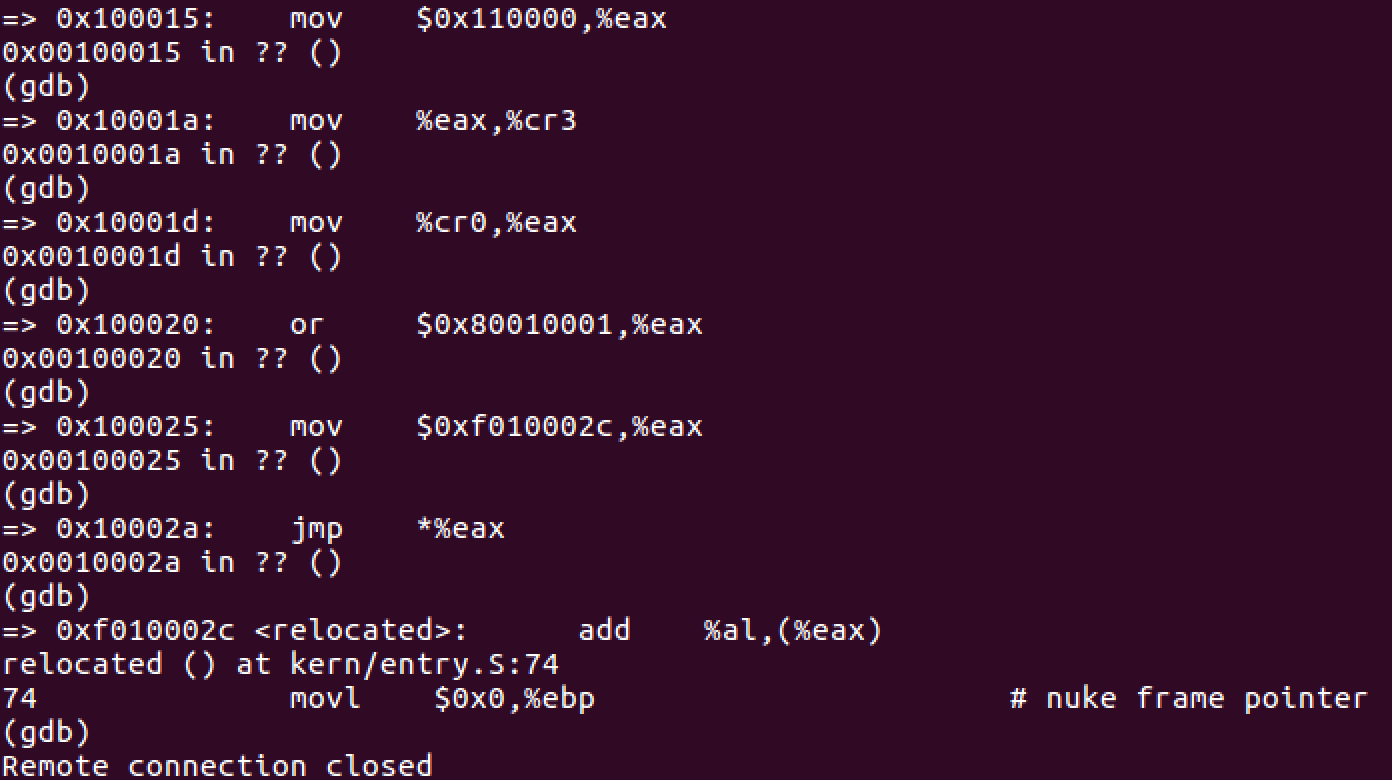
\includegraphics[width=6in]{figures/lab1/ex7.png}
  \caption{GDB截图}\label{fig:lab1:ex7}
\end{figure}

在0x10002a处的jmp指令,要跳到 0xf010002c 处, 然而因为没有分页管理,不会进行虚拟地址映射到物理地址的转化,如图\ref{fig:lab1:fatal},在另一个窗口可以看到错误信息,访问地址超出内存。

\begin{figure}[H]
  \centering
  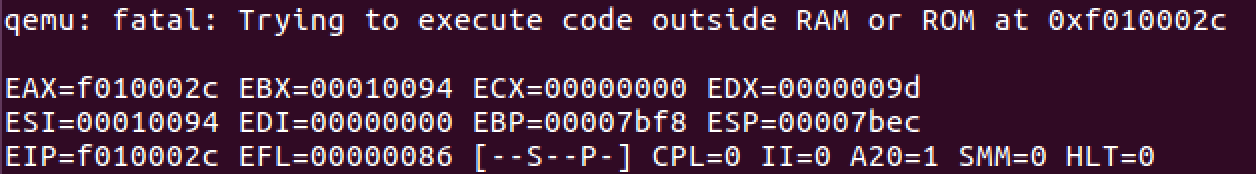
\includegraphics[width=6in]{figures/lab1/fatal.png}
  \caption{错误截图}\label{fig:lab1:fatal}
\end{figure}

\Exercise{完成指定输出''\%o''格式字符串的代码。}

要去实现\%o的格式化输出。在 lib/printfmt.c 可以看到要填写的地方。参考上面 case 'u' 的写法。

\begin{minted}{C}
case 'o':
    num = getuint(&ap, lflag);
    base = 8;
    goto number;
\end{minted}

修改完以后保存,make clean 之后运行,会发现启动以后,如图\ref{fig:lab1:printf},qemu里JOS启动时会出现这样一行字。

\begin{figure}[H]
  \centering
  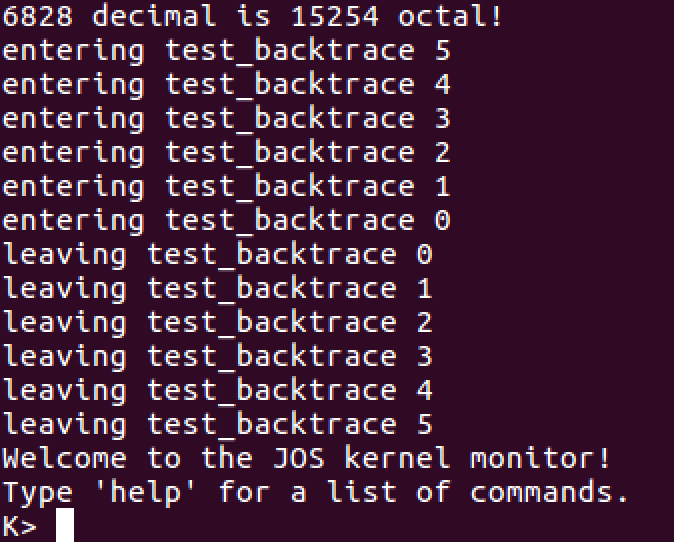
\includegraphics[width=6in]{figures/lab1/printf.png}
  \caption{错误截图}\label{fig:lab1:printf}
\end{figure}

\Exercise{研究内核是在哪初始化堆栈,找出堆栈存放在内存的位置。内核是如何保存一块空间给堆栈的?堆栈指针指向这块区域的哪儿?}

看了几个文件以后,发现在 kern/entry.S 中提到了设置堆指针和栈指针。

\begin{minted}{ASM}
    # Clear the frame pointer register (EBP)
    # so that once we get into debugging C code,
    # stack backtraces will be terminated properly.
    movl    $0x0,%ebp            # nuke frame pointer

    # Set the stack pointer
    movl    $(bootstacktop),%esp
\end{minted}

为了查看堆的位置,所以要使用gdb,同样还是 b *0x10000c 打断点进入 entry。 si 一步步执行,在 0x10002d: jmp *\%eax 之后,下一条指令变为 0xf010002f <relocated>: mov \$0x0,\%ebp。其实地址应该还是 0x10002f,所以这里的 0xf010002f 是因为开启的虚拟地址。

通过 gdb 发现 0xf0100034 <relocated+5>: mov \$0xf0110000,\%esp, 也就是说\%esp也就是bootstacktop的值为0xf0110000。其中 kern/entry.S 的 KSTKSIZE 应该就是堆栈的大小,通过跳转,发现在 inc/memlayout.h 里提到了堆栈。

\begin{minted}{C}
// Kernel stack.
#define KSTACKTOP    KERNBASE
#define KSTKSIZE    (8*PGSIZE)           // size of a kernel stack
#define KSTKGAP        (8*PGSIZE)           // size of a kernel stack guard
\end{minted}

\Exercise{研究 obj/kern/kernel.asm 中 test\_backtrace 向堆栈里压入的信息。}

使用单步调试和 info registers 来查看esp和ebp的变化。

运行test\_backtrace前寄存器如下所示,

{\noindent\small esp            0xf010ffdc    0xf010ffdc\\
ebp            0xf010fff8    0xf010fff8
}

现在需要实现mon\_backtrace()这个函数,需要显示ebp,eip 和 args。ebp是基址指针,eip是返回指令指针。简单实现backtrace,实现效果如下:

{\noindent\small Stack backtrace:
  ebp f0109e58  eip f0100a62  args 00000001 f0109e80 f0109e98 f0100ed2 00000031\\
  ebp f0109ed8  eip f01000d6  args 00000000 00000000 f0100058 f0109f28 00000061
  ...}

代码:

\begin{minted}{C}
int
mon_backtrace(int argc, char **argv, struct Trapframe *tf)
{
        // Your code here.
        int i, j;
        uint32_t *ebp = (uint32_t*)read_ebp();
        uint32_t eip;
        struct Eipdebuginfo info;
        cprintf("Stack backtrace:\n");
        while (ebp != NULL) {
                eip = ebp[1];
                cprintf("  ebp %08x  eip %08x  args", ebp, eip);
                debuginfo_eip(eip, &info);
                uint32_t *args = ebp + 2;
                for (j = 0; j < 5; j ++) {
                        cprintf(" %08x", *(args + j));
                }
                cprintf("\n");
                cprintf("         %s:%d: ", info.eip_file, info.eip_line);
                for (i = 0; i < info.eip_fn_namelen; i++)
                        cprintf("%c", info.eip_fn_name[i]);
                cprintf("+%d\n", eip-info.eip_fn_addr);

                ebp = (uint32_t*)(ebp[0]);
        }
        return 0;
}
\end{minted}

\Exercise{修改上面实现的backtrace,要显示详细的函数地址。可以使用 kern/kdebug.c 的 debuginfo\_eip()。}

在查看debuginfo\_eip时发现其中有一段代码需要填写。这段代码是填写eip\_line。这里用到了写好的二分查找。

\begin{minted}{C}
// Your code here.
stab_binsearch(stabs, &lline, &rline, N_SLINE, addr);
if (lline <= rline) {
  info->eip_line = stabs[lline].n_desc;
} else {
  info->eip_line = 0;
  return -1;
}
\end{minted}

\Exercise{将backtrace嵌入终端中,使其可以被调用。}

只需要修改 kern/monitor.c 的这个部分:

\begin{minted}{C}
static struct Command commands[] = {
    { "help", "Display this list of commands", mon_help },
    { "kerninfo", "Display information about the kernel", mon_kerninfo },
    { "backtrace", "Display a listing of function call frames", mon_backtrace}
};
\end{minted}

至此,Lab1正式完成。

\begin{figure}[H]
  \centering
  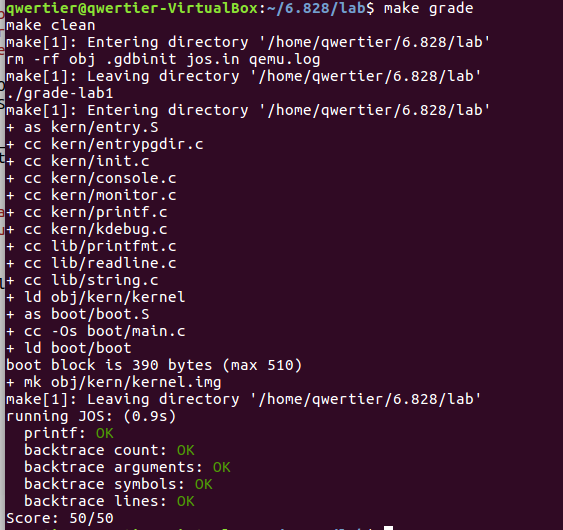
\includegraphics[width=6in]{figures/lab1/finish.png}
  \caption{实验1完成图}\label{fig:lab1:finish}
\end{figure}

\end{ExerciseList}
